\documentclass[11pt,a4paper]{article}
\usepackage[margin=23mm]{geometry}
\usepackage[T1]{fontenc}
\usepackage{lmodern,graphicx,hyperref,fancyvrb,enumitem}
\hypersetup{colorlinks=true,urlcolor=blue,linkcolor=blue}
\setlength{\parindent}{0pt}\setlength{\parskip}{7pt}
\setlength{\emergencystretch}{4em}
\setlist[enumerate]{leftmargin=*,itemsep=5pt}
\title{Blender Optical Schematics\\\large From a fresh download to your first figure}
\author{B. M. Rodriguez-Lara}\date{5 November 2026}
\begin{document}\maketitle
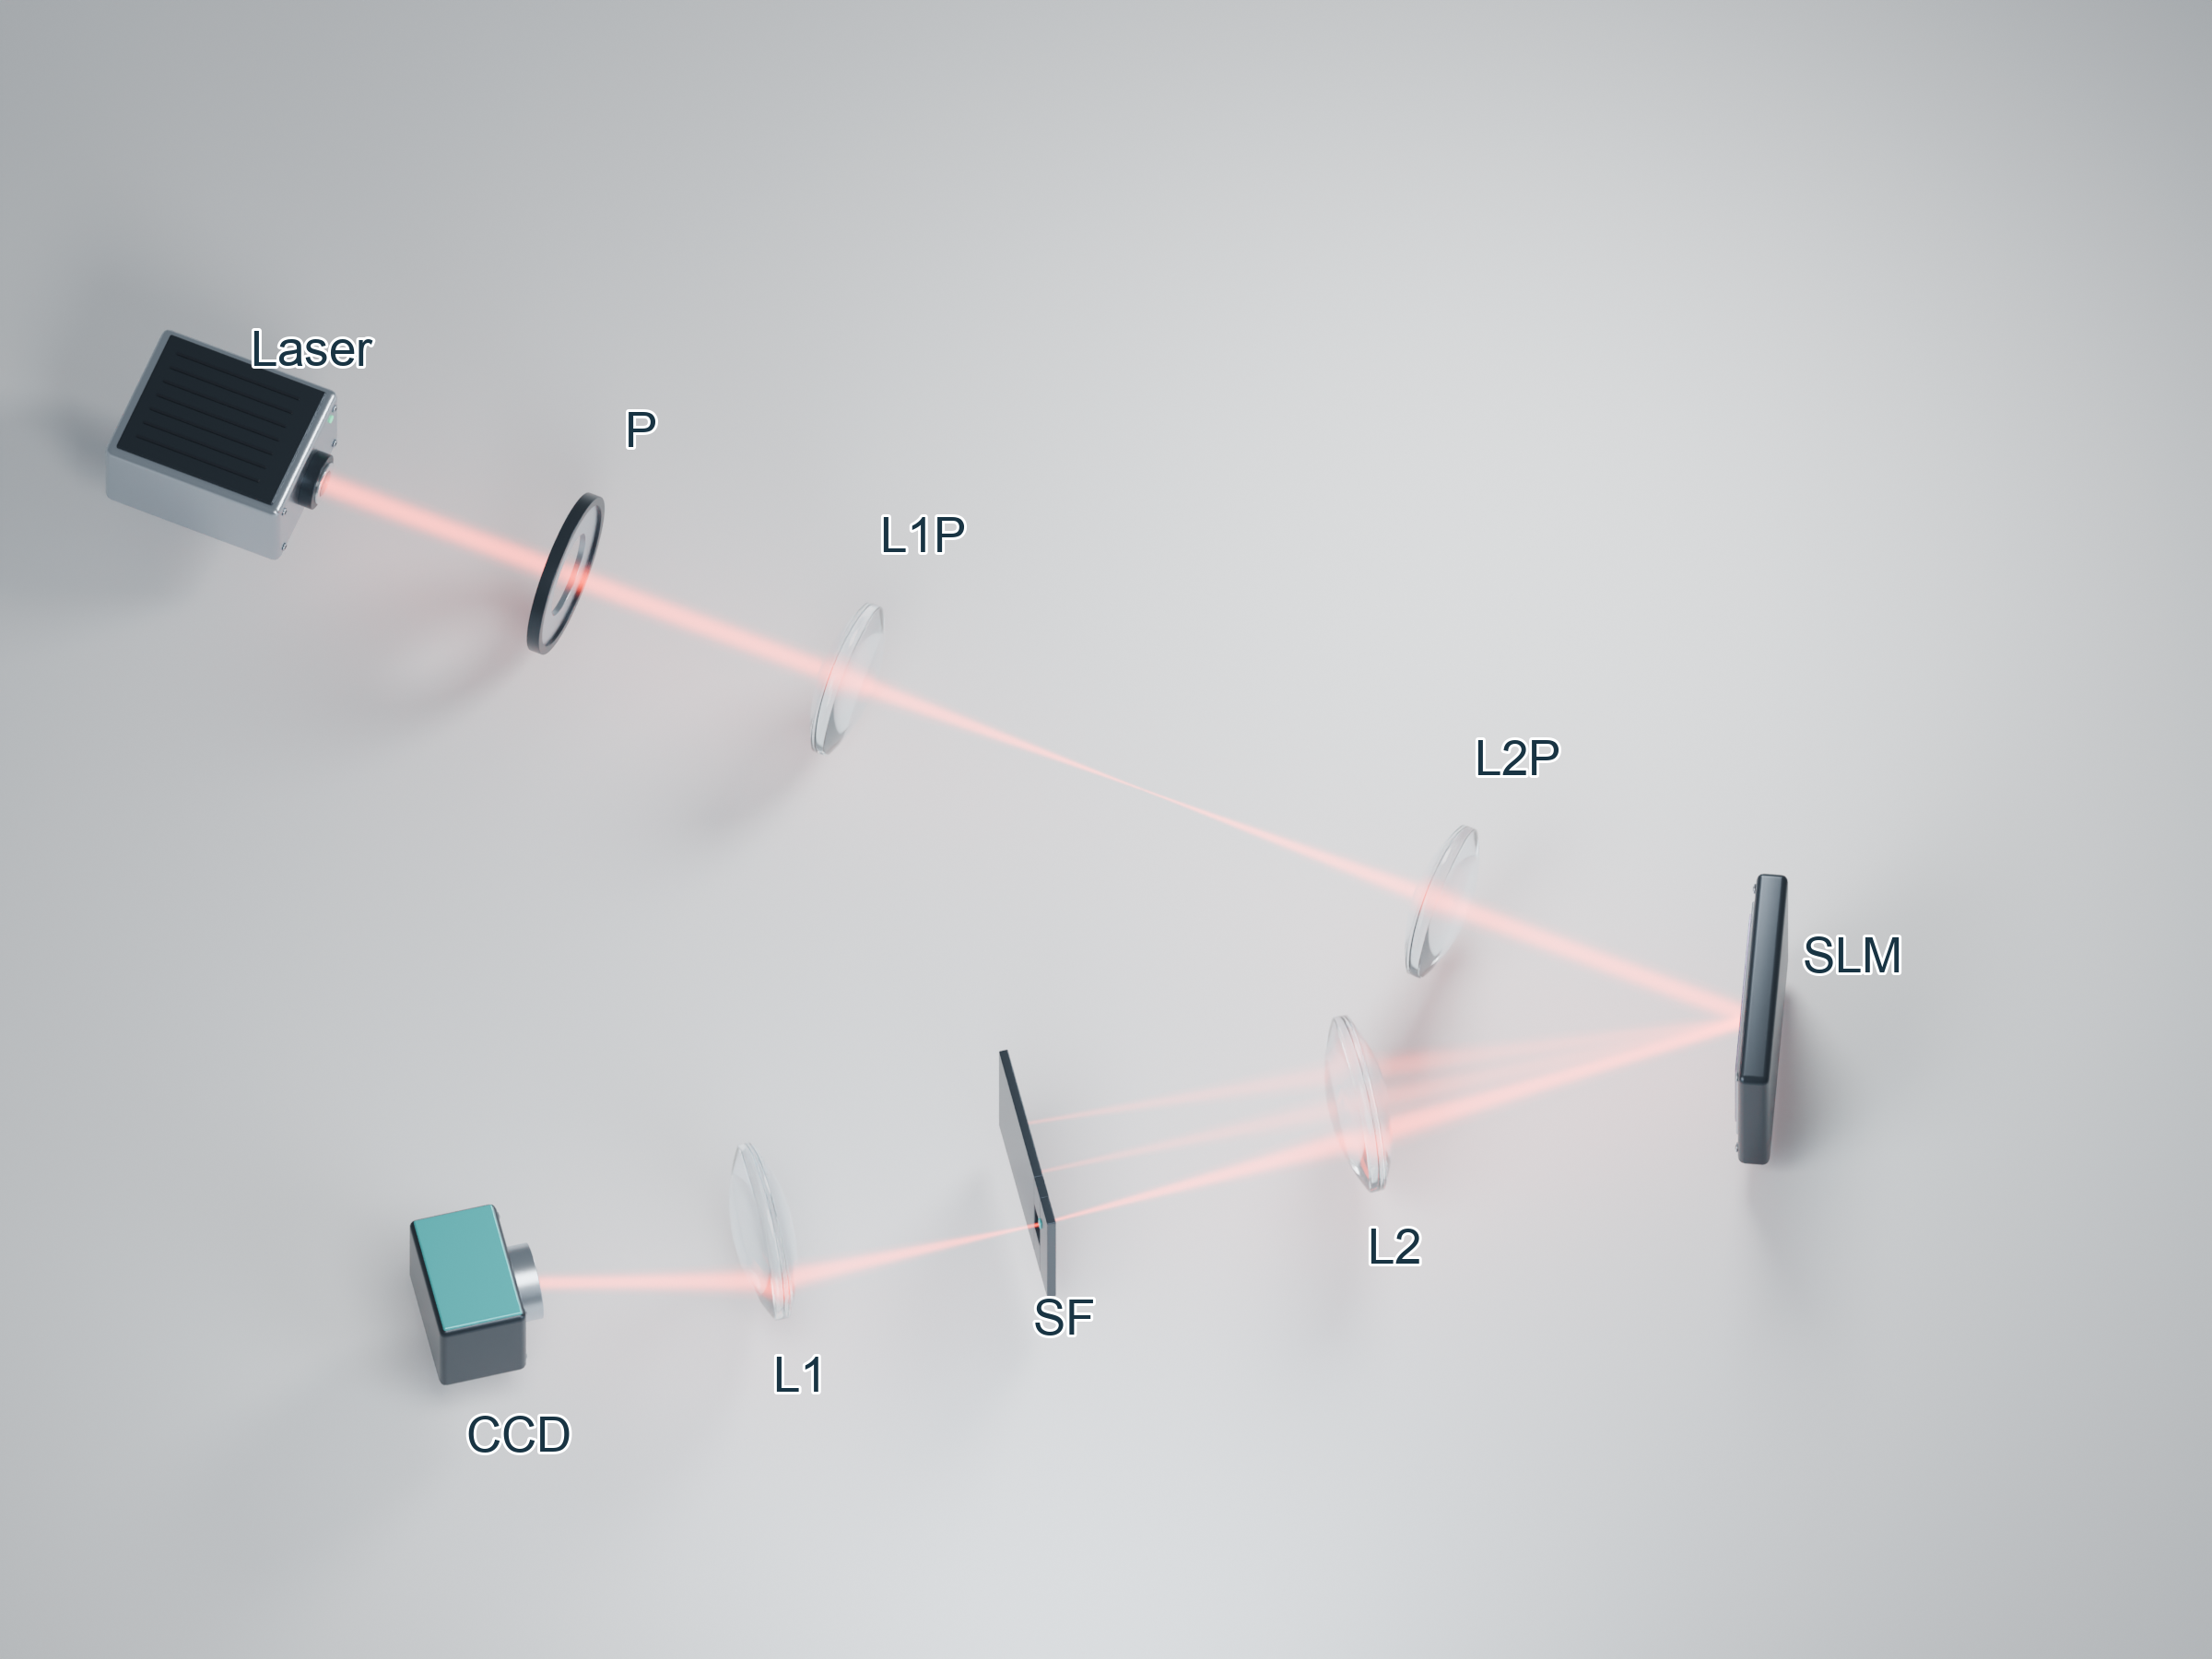
\includegraphics[width=\linewidth,height=.48\textheight,keepaspectratio]{../images/paper-example.png}\par
\medskip
\textbf{What you will make.} A Blender recreation of the optical setup illustrated in the paper, with an editable Blender file, two rendered views and SVGs with editable labels. This image is a reference preview from our later reconstruction, with the supplied SLM hologram and CCD intensity panels beside their instruments. Your first run follows the supplied layout; exact framing may vary because the agent writes the scene builder.

\textbf{What inspired this project.} The basic optical-setup schematic in \url{https://doi.org/10.1103/6ftp-svh8} motivated the development of this Blender library. The paper contains no Blender model. The models and this example were created afterward; they were neither used in nor supplied with that publication. The paper DOI identifies the article, not this library.

No Blender coding experience is assumed. Follow the steps in order. The catalogue image is available separately at \path{images/catalogue-cover.png}.
\clearpage
\section*{1. Install the two applications}
\begin{enumerate}
\item Install Blender from \url{https://www.blender.org/download/}. These assets were prepared with Blender 5.2.3 LTS. Use that version or a compatible newer version; older versions have not been tested.
\item Launch Blender once to finish its initial setup. Confirm that its normal scene window opens. You can close it afterward.
\item Install/open Codex from the official OpenAI application documentation, \url{https://developers.openai.com/codex/app/}, and sign in. Use a local project session that can read files and run Blender. A browser-only conversation without local file/execution access cannot perform this workflow on your computer.
\end{enumerate}
\textbf{Roles.} Blender builds and renders the scene. Codex reads the agent instructions and writes/runs the build script. The supplied agent is a folder of instructions, not a third application or a Blender add-on. No API programming is needed for this walkthrough.
\section*{2. Download and keep the complete project together}
\begin{enumerate}
\item If using GitHub, open this project's repository, choose Code, then Download ZIP. Extract the ZIP. Do not work inside the compressed ZIP. If you received a folder directly, use that complete folder.
\item Put the extracted project in a stable location, for example \path{Documents/OpticalElements/blender-optical-schematics/}. You may rename a downloaded folder ending in \texttt{-main} to \texttt{blender-optical-schematics}.
\item Open that folder in your file browser. You should see the following structure. This folder is called the \textbf{project root} in the remaining steps.
\end{enumerate}
\begin{Verbatim}[fontsize=\small]
blender-optical-schematics/
  README.md
  library/                  Blender asset files
  agent/                    The agent's own folder
    README.md
    install.py
    setup-to-blender/
      SKILL.md
      agents/
      references/
  examples/paper-setup/      Prompt and starting layout
  scripts/                  Reusable beam helper
  images/                   Catalogue and example preview
  docs/                     This PDF and its LaTeX source
\end{Verbatim}
\textbf{Checkpoint.} Keep \texttt{library/} and \texttt{agent/} here. Do not move them into Blender's application folder or split them across unrelated locations. All later relative paths start at this project root.
\clearpage
\section*{3. Register the library in Blender}
These steps let you browse and drag components by hand. The agent's build script can also read the same library files directly.
\begin{enumerate}
\item Open Blender and open Preferences (normally Edit, then Preferences; on some macOS versions use the Blender application menu).
\item Find Asset Libraries. Depending on Blender version it is a separate preferences section or appears under File Paths.
\item Click the plus/add button. Browse to the project root and select its \texttt{library} folder. Select the folder, not an individual \texttt{.blend} file and not the \texttt{agent} folder.
\item Give it a recognizable name such as \texttt{Optical Schematics}. Save preferences if automatic saving is disabled.
\item In a Blender editor area's upper-left editor-type menu, choose Asset Browser. Select \texttt{Optical Schematics} in its library selector. If categories are empty, select All to see every asset.
\item Drag one collection into a fresh scene to confirm that it appears. You can discard this test scene. Do not save changes over a file inside \texttt{library/}.
\end{enumerate}
\textbf{Checkpoint.} You can see optical components in the Asset Browser. Schematic assets use 1 Blender unit = 10 mm, with illustrative geometry. Catalogue thumbnails normalize sizes for legibility; use the source collection scale in your scene.
\section*{4. Open the correct folder in Codex}
\begin{enumerate}
\item Use Codex's project/folder selection to open the \texttt{blender-optical-schematics} folder you saved in Step 2. Choose the project root, not \texttt{library/}, \texttt{agent/} or the parent folder containing both optical projects.
\item Start a chat attached to that local folder. Select local work if your interface offers a choice between local and remote execution.
\item Paste this readiness check. It does not ask Codex to generate the figure yet.
\end{enumerate}
\begin{Verbatim}[fontsize=\small]
Check that this project contains library/, agent/, and
examples/paper-setup/. Locate Blender on this computer and
report its version. Do not generate a figure yet. If any
required file or application is missing, tell me exactly
what I need to fix before continuing.
\end{Verbatim}
\textbf{Checkpoint.} Codex confirms the three folders and finds Blender. If Blender is not on the system search path, give its executable location. On macOS it is commonly \path{/Applications/Blender.app/Contents/MacOS/Blender}. On Windows, locate \texttt{blender.exe} inside the installed Blender folder; the versioned folder name varies.
\clearpage
\section*{5. Put the agent in place}
\textbf{Recommended first run.} Leave the complete \texttt{agent/} folder where it is. No extra installation is required when you call it by file path in Step 6. This avoids hidden-folder setup and automatic-discovery issues.

\textbf{Optional named call.} If you want to type \texttt{\$setup-to-blender}, install a project-local copy. In Codex, paste:
\begin{Verbatim}[fontsize=\small]
Install this project's agent by running agent/install.py
with an available Python interpreter from this project
root. Do not install globally or overwrite a different
existing agent. Report the installed SKILL.md path.
\end{Verbatim}
The installer uses only standard Python. If Python is unavailable, the manual alternative is to copy the whole \texttt{agent/setup-to-blender} folder into \texttt{.agents/skills/} under this same project. Codex can perform that copy if you ask. The installed path must be:
\begin{Verbatim}[fontsize=\small]
blender-optical-schematics/.agents/skills/setup-to-blender/SKILL.md
\end{Verbatim}
The dot-prefixed \texttt{.agents} folder is normally hidden. Keep the visible \texttt{agent/} folder as the original distribution. After optional installation, start a new chat in the same project. If the named skill is still not recognized, use the direct call below; it does not depend on skill discovery.
\section*{6. Generate the example inspired by the paper}
For the first run, use the supplied list and layout without adding files. Paste this exact request in the project chat:
\begin{Verbatim}[fontsize=\small]
Read agent/setup-to-blender/SKILL.md and follow it to carry
out examples/paper-setup/prompt.md. Use this project only.
Generate the paper-setup example now, not just a plan.
Use the supplied layout assumptions and both bundled
SLM/CCD image panels. Save to a new dated Figures folder; preserve
existing files and libraries. Run Blender, inspect both
views, and give me links to the Blender file, renders,
paired SVGs and the validation/assumptions notes.
\end{Verbatim}
If the named skill is installed, the shorter equivalent is:
\begin{Verbatim}[fontsize=\small]
Use $setup-to-blender to execute
examples/paper-setup/prompt.md and generate the example.
\end{Verbatim}
Codex writes the scene plan and build script, runs Blender, exports the figures and checks them. Rendering can take time; wait for a completion report. Respond to any application access request only after checking that it concerns this project and Blender. Do not close the running task before it finishes.
\clearpage
\section*{7. Find and open your finished figure}
The agent selects an unused figure number using your local date. A typical output folder looks like this; the date and filenames may differ, so use the links in its completion message.
\begin{Verbatim}[fontsize=\small]
Figures/YYYY-MM-DD-FIgNN/
  build.py                  Repeatable Blender build
  setup.json                Interpreted scene plan
  ...blend                  Editable Blender scene
  renders/                  Perspective and plan PNGs
  svg/                      Lettered/unlettered SVG pairs
  README.md                 Assumptions and checks
\end{Verbatim}
\begin{enumerate}
\item Double-click the \texttt{.blend} file to open it in Blender. It is the editable result, not a library source file.
\item Open the PNGs in \texttt{renders/} to review the perspective and overhead views. A window showing only a default cube is not a completed result.
\item Open a lettered SVG in a vector editor to edit text. The optics are an embedded raster render; the lettering is vector text. The unlettered SVG omits the lettering layer. Default output width is 86 mm.
\item Read the figure README. Check the optical sequence, labels, assumptions and reported validation before using the image in a publication.
\end{enumerate}
\textbf{Expected topology.} Laser, circular pupil P, L1P, L2P, reflective SLM, L2, filter SF, L1, CCD. The selected +1 order continues through SF; rejected orders end there. P is not a polarizer. No extra beam splitter is implied. The documented figure labels put L2 nearest SLM and L1 nearest CCD; earlier notes report conflicting manuscript prose.

\textbf{What is assumed.} Positions and mounting choices are authored layout assumptions, not measurements. Focal lengths are unknown. The experimental pupil and filter openings are assumed to be 4 mm and 1 mm. Gaussian envelopes are visual guides, not diffraction simulations. Mechanical fit is not certified.
\section*{8. Add your own sketch or data images later}
Create \texttt{inputs/paper-setup/} inside the project and place your lawful sketch/PDF and any SLM/CCD reference PNGs there. Tell Codex the exact filenames and which component each image belongs to. Ask for a new figure variant rather than overwriting the first run. The example includes two PNGs in \path{examples/paper-setup/reference-images/}: \texttt{slm\_hologram.png} beside SLM and \texttt{ccd\_intensity.png} beside CCD. They are supplied reference imagery, not Blender simulation results. Their source and existing rights are recorded in that folder's README. The full paper PDF is not bundled. Without a supplied sketch the agent reconstructs the documented topology and must not claim to have checked the original drawing.
\clearpage
\section*{9. If something does not work}
\begin{description}[leftmargin=0pt,style=nextline]
\item[Codex cannot find SKILL.md or layout.json.] You probably opened the wrong folder or did not extract the ZIP. Return to Step 2, then open the project root in Codex. Confirm \texttt{agent/setup-to-blender/SKILL.md} exists.
\item[The agent is not listed.] Use the direct file-path call in Step 6. If using the optional installer, verify the exact hidden-folder path in Step 5 and start a new project chat.
\item[The Blender Asset Browser is empty.] Confirm you registered the \texttt{library/} folder containing the \texttt{.blend} files. Select the correct library and All categories. Reopen Blender if needed. Registration affects manual browsing; a script can still append directly from existing library files.
\item[Blender is not found.] Install and launch it once. Give Codex its actual executable path. Do not supply a shortcut or the containing folder when an executable is requested.
\item[Python or Pillow is missing.] Ask Codex to identify the missing dependency and use a project-local environment for the exporter. Blender has its own Python for scene builds. The optional installer needs standard Python, but the direct file-path agent call does not need the installer.
\item[Codex only returns a plan.] Paste: ``Continue and generate the files. Run Blender, export both views and paired SVGs, then inspect and link the results.'' If it cannot execute locally, switch to a local project session or follow its reported installation fix.
\item[Rendering is slow.] Ask for a separate preview at 1000 by 800 pixels and 12 samples. Once it looks right, request the final 2000 by 1600 images with 40 samples. Do not present the preview as the final render.
\item[An SLM or CCD panel is missing.] Confirm both bundled reference PNGs exist. Ask the agent to load them, pack the textures and inspect both camera views. Do not substitute invented data.
\item[Labels, apertures or beams look wrong.] Ask for a corrected variant and state the specific discrepancy. Moving an optic does not automatically reroute its beam; both need updating in the scene plan. Preserve the original result for comparison.
\end{description}
\section*{Sources, licenses and editable documentation}
The agent installation convention is documented at \url{https://developers.openai.com/codex/skills/}. Blender's library preferences are documented at \url{https://docs.blender.org/manual/en/5.4/editors/preferences/asset_libraries.html}. Menu placement varies by version.

Original code uses MIT; original authored models and documentation use CC BY 4.0. See LICENSE and \texttt{docs/provenance.md} for exclusions. See the following section for the library DOI and citation formats.

This guide's editable source is \texttt{docs/user-guide.tex}. To rebuild it, run \texttt{pdflatex user-guide.tex} twice from \texttt{docs/}. The example image is \texttt{images/paper-example.png}. The full catalogue is separate; there is no collection index in this guide.

\clearpage
\section*{10. How to cite}
When using this library to prepare a figure, cite the archived release you used. For version v0.1.2, use:

Rodriguez-Lara, B. M. (2026). \textit{Blender Optical Schematics} (Version v0.1.2) [Computer software]. Zenodo.\newline
\url{https://doi.org/10.5281/zenodo.23994376}

\textbf{Which DOI?} The DOI above identifies the fixed v0.1.2 release, published on 6 November 2026. Prefer it when documenting reproducible work. The all-versions DOI, \url{https://doi.org/10.5281/zenodo.23993947}, identifies the project across releases; use it for a general reference to the library. For a future release, use that release's own citation metadata rather than retaining the v0.1.2 DOI.

\subsection*{BibTeX for LaTeX}
Copy this entry into your bibliography \texttt{.bib} file, or use the supplied \path{docs/citations/schematics.bib}. The \texttt{@misc} entry works with traditional BibTeX styles; version information is included in the note.
\begin{Verbatim}[fontsize=\small]
@misc{rodriguez_lara_2026_optical_schematics,
  author    = {Rodriguez-Lara, B. M.},
  title     = {{Blender Optical Schematics}},
  year      = {2026},
  publisher = {Zenodo},
  doi       = {10.5281/zenodo.23994376},
  url       = {https://doi.org/10.5281/zenodo.23994376},
  note      = {Version v0.1.2. Computer software}
}
\end{Verbatim}
In your manuscript, use \verb|\cite{rodriguez_lara_2026_optical_schematics}| and compile with your normal bibliography workflow.

\subsection*{Other formats and reference managers}
\begin{itemize}[leftmargin=*,itemsep=3pt]
\item \textbf{RIS:} import \path{docs/citations/schematics.ris} into a reference manager such as Zotero or EndNote.
\item \textbf{CSL-JSON:} use \path{docs/citations/schematics.csl.json} with tools supporting Citation Style Language data.
\item \textbf{Plain text:} copy \path{docs/citations/schematics.txt} and adapt the formatting to your journal's style.
\item \textbf{CFF:} \path{CITATION.cff} in the project root provides machine-readable citation metadata for GitHub and other tools.
\end{itemize}
\textbf{Cite the library for the Blender assets.} Use the library DOI above when using these models. Cite the paper at \url{https://doi.org/10.1103/6ftp-svh8} only when referring to its optical setup or scientific results. Its basic schematic inspired this project; the article contains no Blender model. The models were created afterward and were neither used in nor supplied with the publication. Library citation does not replace the attribution required by CC BY 4.0 for reused models, figures and documentation.

\end{document}
